\chapter*{The tambora.org data series edition}
\addcontentsline{toc}{chapter}{The tambora.org data series edition}
\textbf{Rüdiger Glaser, Michael Kahle \& Rafael Hologa}\\
Albert-Ludwigs-University Freiburg, Institute for Environmental Social Sciences and Geography, Department of Physical Geography
\vspace{0.75cm}

The tambora.org data series has been established to offer all contributors of the collaborative research environment (CRE) tambora.org a convenient opportunity to publish comprehensive data collections. To bridge digital and analog purposes the data collections are not only stored in the classical analog format but also digitally. This guarantees that the enormous effort of finding, collecting and coding relevant climatic, societal and environmental information from different sources and archives is made visible and citable.

For the dissemination of coded historical and modern information and documents to manifold academic disciplines, the interested public, stakeholders and the media the digital data storage plays a key role. Moreover, it stimulates ongoing research to discover unexplored and hidden treasures in historical documents. Last but not least it promotes principles of transparent and open science.

Each entry comprises a basic text excerpt, a time and location code and a short content coding for easy orientation and initial interpretation. The presented format of tambora.org data series opens useful digital functions likewise text search or hyperlinks. For detailed and complete content-related coding information and the full range of classified indices there is an object identifier to enter the CRE tambora.org (c.f. fig. 1). The standardized data format of the tambora.org data series allows a comparison of data values and content across several volumes.
\vspace{0.25cm}\\
\begin{figure}[H]
	\begin{center}
 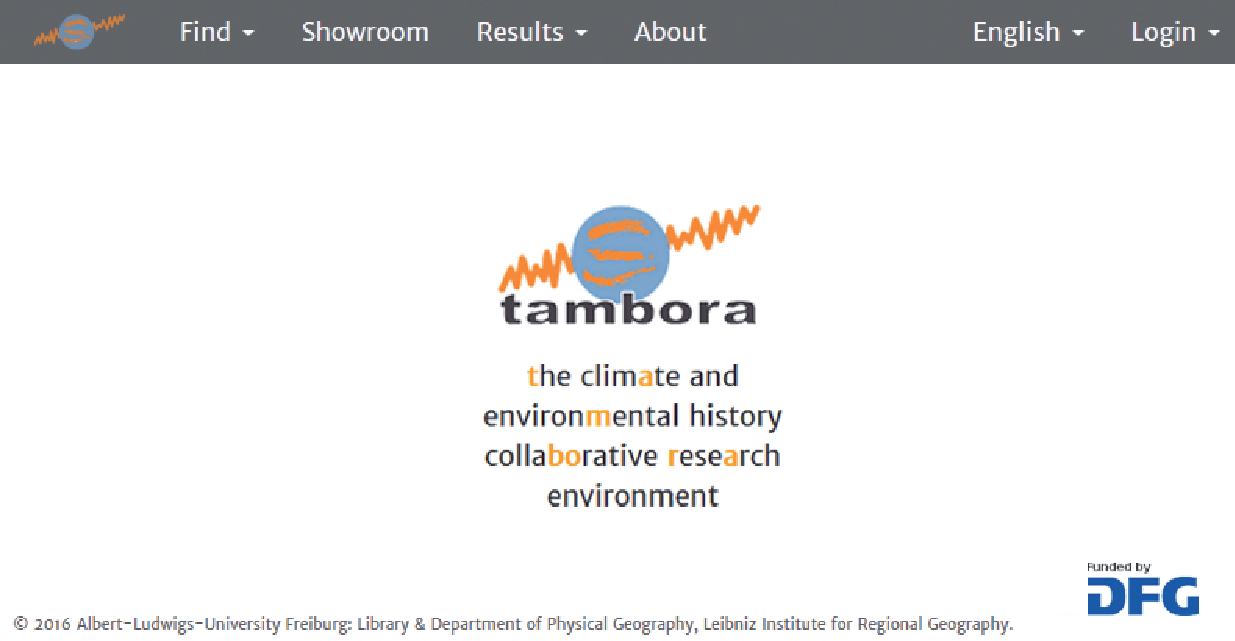
\includegraphics[width=0.6\textwidth]{fig/notes/startpage.pdf}
 \caption*{\textit{Figure 1:} Typical workflow of tambora.org to create valuable data sets out of historical documents.}
 \end{center}
\end{figure}
The tambora.org data series is also meant to be a source of inspiration and further research, encouraging publications based on deeper investigations of existing data sets as well as additional contributions to tambora.org. Thereby, the editors aim at the continuous extension and the effective long-term use of the stored data. 
\\\\
\textbf{Development of the tambora.org data series – from analog to digital}
\vspace{0.25cm}\\
The analysis of environmental and societal change on the basis of written documents is interconnected with the general development of sources and information documentation. History – in this context defined as the period which can be analyzed on the basis of human documents - started with hand-written sources before Guttenberg’s fundamental invention of the printing press which led to a “quantum jump of information”. We have experienced a similar kind of innovation and increase in information since the introduction of the internet in the 1990s. The documentation and publication of sources and relevant information reflects this long historical path.

An outstanding example of the edition of medieval sources and annals can be seen in the Monumenta Germaniae Historica (MGH). The MGH started in the early 19th century with the edition of original primary sources of both chronicles of the middle ages, following the principles of historical sciences. The Collection of Weikinn stands in the tradition of this kind of classical analog data format (Börngen\&Tetzlaff, 2002). The same is true for the collection of weather and environmental sources and data for Franconia, Saxony and Thuringia for the period 1500-1699 (Glaser\&Militzer. 1993). These classical editions have been transformed into digital versions, the latter forming part of tambora.org’s CRE. Such editions have been digitized and are accessible via digital repositories (e.g. www.mgh.de). These initiatives illustrate the paradigm shift to publish analog textbooks in electronical format. This offers new opportunities like search functions and provides handy options to store, recombine, and interactively explore the texts. In the meantime many data portals and repositories are established (e.g. Cram et. al. 2015), supported by modern information technologies which enable 24/7 access from all over the world. All of these are closely connected to a synoptic analysis by the international scientific community, leading to comprehensive findings (e.g. Camenisch et al (2016), Böhm et al (2016), Himmelsbach et al. (2016)).

The newest developments in this field are e-research technologies like CREs which integrate team working environments. These enable contributors to not only sustainably store and exchange data, methods and results in a multifold manner, but also to collectively evaluate them. Additionally, it offers complex ownership and publication options and access rights. Tambora.org feels committed to the ideals of transparency, transferability and validation and intends to highlight and support the scientific adding value process. Given the fact of manifold data handling and publishing formats tambora.org combines the advantages of both analog and digital editions, cordially inviting the scientific community to use the digital tools and options of the CRE tambora.org.
\\\\
\textbf{The tambora.org workflow}
\vspace{0.25cm}\\
The CRE of tambora.org reflects the complex workflow of historical climatology and neighbouring fields of environmental science. As illustrated in figure 2, tambora.org’s workflow starts with source research and continues with the digitalization of the discovered documents (e.g. sources, historical newspapers, weather diaries, printed graphs, flood marks and paintings). It proceeds with the transcription and translation of the paleographic material, if necessary. Based on this, critical source analysis is conducted as a prerequisite for the precise analysis, coding and classification of the raw material.  Therefore tambora.org offers a wide range of different content-related coding options (c.f. figure 3) as well as tools to define spatial and temporal extensions for given analysis purposes (e.g. for the description of historical weather events). Because of tambora.org’s development the workflow primarily complies the needs of historical and environmental science and research, but it can also be adjusted to requirements of other fields that work with coded historical material.
\vspace{0.25cm}\\
\begin{figure}[H]
	\begin{center}
 \includegraphics[width=0.5\textwidth]{fig/notes/workflow.pdf}
 \caption*{\textit{Figure 1:} Typical workflow of tambora.org to create valuable data sets out of historical documents.}
 \end{center}
\end{figure}
As coding of phenomena includes the derivation of numerical indices, it enables the derivation of manifold temporal and spatial patterns (e.g. weather patterns in time). Finally, the coded material can be published as readable data set as well as in a more technical, machine-processable format. Both media meet the need for scientific communication and guarantee a permanent identification via the international citation standard doi and the usage of an adequate Creative-Commons-License.
\\\\
\textbf{The tambora.org coding scheme}
\vspace{0.25cm}\\
The wide-ranging coding scheme indicated in figure 3 reflects the first two hierarchal levels. It shows the fundamental tree structure and the logical and hierarchal order of the content-related coding classes. The actual coding scheme is based on a long interactive and still on-going creative process (Glaser, 1996, Riemann et al, 2016). It requires permanent revisions and extensions into new fields depending on source material.
\begin{figure}[H]
	\begin{center}
 \includegraphics[width=0.75\textwidth]{fig/notes/coding_tree.pdf}
 \caption*{\textit{Figure 2:} The coarse structure respectively the first two hierachle levels of the coding treee for tagging content-related information.}
 \end{center}
\end{figure}
Generally, there are seven coding themes– the most frequently used main categories. Each of them divides into subclasses which are again differentiated into more detailed parameters and aspects. All in all these around 300 different classes and aspects with related indices and up to seven levels of specification are available for deeper content-related coding analysis. Thus, the categories at high hierarchal levels represent very general and more abstract content-related classes, while on deeper levels the degree of specification and differentiation are defined more accurately. This allows a specific level of refinement according to the precision of the source. The coding scheme is the outcome of a long process and the expertise of many contributors over decades- and is still an ongoing process, especially if new data from a different cultural context or further scientific subjects are integrated.
\\\\
\textbf{The formal structure of the tambora.org data series}
\vspace{0.25cm}\\
The formal structure of the data sets comprises a time-stamp, a spatial-stamp and a content-related coding (according to the coding tree, c.f. figure 3). Timing for phenomena in this data series is given as a single date string and not only represents the beginning, but also the duration in varying precision (e.g. day, month or year or more unspecific periods and phases like “for longer times, since last summer”). The spatial position is given by the name of a location and can include points, lines or areas. It can also be unspecified or in a certain regional context, like “on the way from Damascus to Egypt”, or “the Nile”, or “Golan Heights”. In the appendix only the latitude and longitude centroid is listed for each location name. The content-related information of a quote can cover single categories of the coding tree or a combination of them.  So, an apple-blossom can be classified using a class of the phenological branch in combination with one of the biological branch of the coding tree.
\begin{figure}[H]
	\begin{center}
 \includegraphics[width=0.7\textwidth]{fig/notes/description.pdf}
 \caption*{\textit{Figure 3:} Interpreteting scheme to gather the coded information of citations.}
 \end{center}
\end{figure}
The degree of content-, space- and time-related coding depends on the analytical focus intended by the interpreter, thus shaping the form of each data set. The quote as derived from the transcription and translating process of the author(s) gives additional insights into the creators’ intention and zeitgeist. As the author(s) may proceed working on the data set for further refinement and additions it is always worth to visit tambora.org. This present edition reflects the current snapshot of tambora.org’s workflow. The actual codification is based on the specific needs of the underlying project. There are further information’s in the text which can be coded or refined more detailed. On tambora.org all readers are highly welcome to contribute for these reasons. Please contact the editors.
\\\\
\textbf{Declaration}
\vspace{0.25cm}\\
The Editors thank the Deutsche Forschungsgemeinschaft (DFG) for funding the research projects HISKLID Core, Vorderer Orient (GL 358/8-1), Transrisk (GL 358/12-1, GL 358/15-1) and tambora.org (BE 5282/2-2, GL 358/9-1) which can be seen as a prerequisite for this tambora.org data series.
\\\\
\textbf{References}
\vspace{0.25cm}\\
Böhm, O.; Jacobeit, J.; Glaser, R. \& K.-F. Wetzel (2015): Flood sensitivity of the Bavarian Alpine Foreland since the late Middle Ages in the context of internal and external climate forcing factors. In: Hydrology and Earth System Sciences, 19: 4721-4734.\\
Börngen, M. \& G. Tetzlaff (Eds) (2002) Quellensammlung zur Hydrographie und Meteorologie Band I. Curt Weikinn. Quellentexte zur Witterungsgeschichte Europas von der Zeitwende bis zum Jahr 1850. S. 728.\\
Camenisch, C.; Keller.; K. M.; Salvisberg, M.; Amann B.; Bauch M.; Blumer S.; Brázdil R.; Brönnimann S.; Büntgen U.; Campbell B. M. S.; Fernández-Donado L.; Fleitmann D.; Glaser R.; González-Rouco F.; Grosjean M.; Hoffmann R. C.; Huhtamaa H.; Joos F.; Kiss A.; Kotyza O.; Lehner F.; Luterbacher J.; Maughan N.; Neukom R.; Novy T.; Pribyl K.; Raible C. C.; Riemann D.; Schuh M.; Slavin P.; Werner J. P. \& O. Wetter (2016): The early Spörer Minimum – a period of extraordinary climate and socio-economic changes in Western and Central Europe. In: Climate of the Past: 1-33. Doi: 10.5194/cp-2016-7.\\
Cram, T.; Compo, G.; Yin, X.; Allan, R.; McColl, C.; Vose. R.; Whitaker, J.; Matsui, N.; Ashcroft, L.; Auchmann, R.; Bessemoulin, P.; Brandsma, T.; Brohan, P.; Brunet, M.; Comeaux, J.;Crouthamel, R.; Gleason, B.; Groisman, P.; Hersbach, H.; Jones, P.; Jonsson, T.; Jourdain, S.; Kelly, G.; Knapp, K.; Kruger, A.; Kubota, H.; Lentini, G.; Lorrey, A.; Lott, N.; Lubker, S.; Luterbacher, J.; Marshall, G.; Maugeri, M.; Mock, C.; Mok, H.; Nordli, Ø.; Rodwell, M.; Ross, F.; Schuster, D.; Srnec, L.; Valente, M.; Vizi, Z.; Wang, X.; Westcott, N.; Woollen, J. \& S. Worley (2015) The international surface pressure databank version 2. Geoscience Data Journal 2, 1: 31–46.\\
Glaser, R. \& S. Militzer (Eds)(1993): Wetter-Witterung-Umwelt Aufzeichnungen und Daten aus Franken, Sachsen, Sachsen-Anhalt und Thüringen 1500-1699. In: Materialien zur Erforschung früher Umwelten, 2. Geographisches Institut der Universität Würzburg.\\
Glaser, R. (1996): Data and Methods of Climatological Evaluation in Historical Climatology. In: Historical Social Research, 21, 4: 56-88. Retrieved from http://www.jstor.org/stable/20756093.\\
Himmelsbach, I., Glaser, R., Schönbein, J., Riemann, D. \& B. Martin (2015): Reconstruction of flood events based on documentary data and transnational flood risk analysis of the upper Rhine and its French and German tributaries since AD 1480. In: Hydrology and Earth System Sciences; 19: 4149-4164. Doi: 10.5194/hess-19-4149-2015.\\
Riemann, D., Glaser, R., Kahle, M., \& S. Vogt (2016): The CRE tambora.org – new data and tools for collaborative research in climate and environmental history. In: Geoscience Data Journal, 2,2: 63–77. Doi: 10.1002/gdj3.30.\\

\vspace*{\fill}
\noindent
\textbf{How to cite this article:}\\
Glaser, R; Kahle, M. \& R. Hologa (2017) The tambora.org data series edition. In: \ExecuteMetaData[variables.tex]{eds} \ExecuteMetaData[variables.tex]{volume}.\\
\href{dx.\ExecuteMetaData[variables.tex]{doinotes}}{\ExecuteMetaData[variables.tex]{doinotes}}